\documentclass[hyperref=unicode]{beamer}

\usepackage[absolute,overlay]{textpos}
\usepackage{graphicx}
\usepackage{adjustbox}
\usepackage{chemfig}
\usepackage[version=4]{mhchem}
\usepackage{wrapfig}
\usepackage{multirow}
\adjustboxset*{center}
\usepackage{caption}
\usepackage{chemformula}
\usepackage{elements}
\usepackage{chemfig}

%dělení slov
\usepackage{ragged2e}
\let\raggedright=\RaggedRight
%konec dělení slov

\usepackage{fontspec}
\usepackage{unicode-math}

\usepackage{polyglossia}
\setdefaultlanguage{czech}

\def\uv#1{„#1“}

\mode<presentation>{\usetheme{Madrid}}
\DefineNamedColor{named}{pozadi}{RGB}{200,200,200}
\usecolortheme{crane}

\setbeamertemplate{footline}[frame number]

\addtobeamertemplate{frametitle}{
	\let\insertframetitle\insertsectionhead}{}
\addtobeamertemplate{frametitle}{
	\let\insertframesubtitle\insertsubsectionhead}{}

\makeatletter
\CheckCommand*\beamer@checkframetitle{\@ifnextchar\bgroup\beamer@inlineframetitle{}}
\renewcommand*\beamer@checkframetitle{\global\let\beamer@frametitle\relax\@ifnextchar\bgroup\beamer@inlineframetitle{}}
\makeatother
\setbeamercolor{section in toc}{fg=blue}
\setbeamertemplate{section in toc shaded}[default][100]

\title[Crisis]
{Chemická vazba}

\subtitle{Rezonanční struktury, atomové a molekulové orbitaly, hybridizace}

\date{}

\titlegraphic{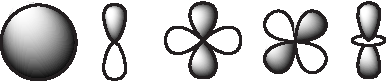
\includegraphics[keepaspectratio,width=11cm]{orbitals-title.pdf}}

\begin{document}
\frame{\titlepage}

\frame{
	\frametitle{Formální náboj}
	\begin{itemize}
	\item Rozdíl mezi počtem valenčních elektronů ve volném atomu a valenčních elektronů ve vázaném atomu.
	\item Záporný náboj je umístěn na nejelektronegativnějším atomu.
	\item Součet formálních nábojů všech atomů v molekule je roven jejímu náboji.
	\item \ce{H3O^+}: H: 0; O: +1
	\item \ce{H3CO^-}: H: 0; C: 0; O: -1
	\end{itemize}
}

\frame{
	\frametitle{Rezonanční struktury}
	\begin{itemize}
	\item Popisují polohu elektronů v molekulách.
	\item Vyjadřují jednotlivé limitní stavy.
	\end{itemize}
	\begin{figure}
		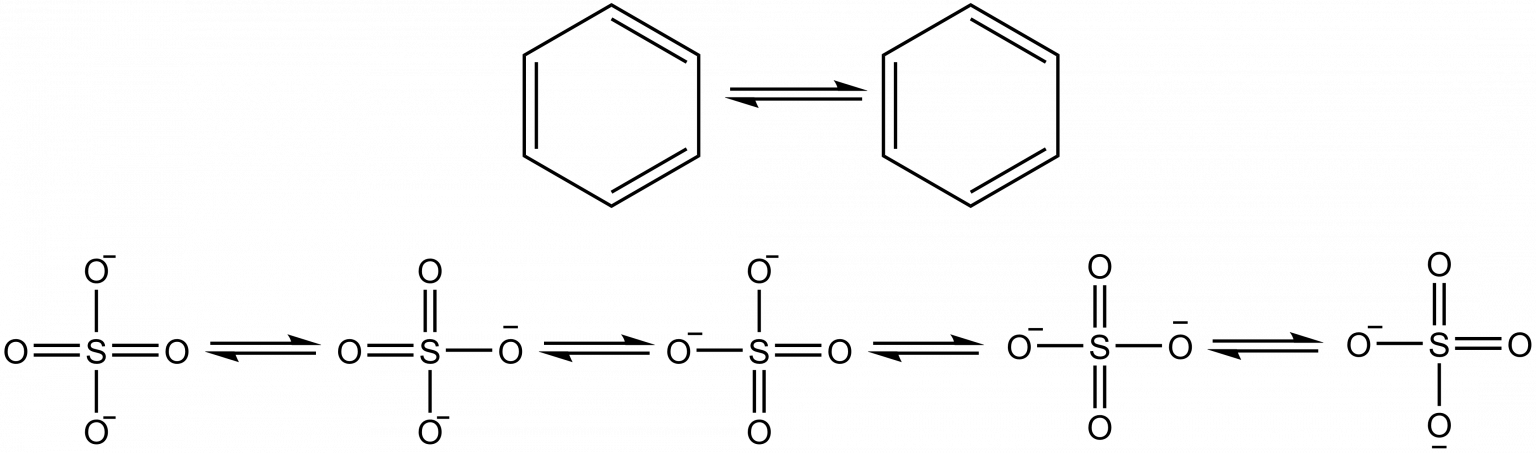
\includegraphics[width=\textwidth]{resonance.png}
	\end{figure}
}

\frame{
	\frametitle{Atomové orbitaly}
	\begin{itemize}
	\item Funkce popisující prostorové rozložení pravděpodobnosti výskytu elektronu.
	\item Orbitaly jsou popsány třemi kvantovými čísly.
	\begin{itemize}
	\item Hlavní kvantové číslo (n) - popisuje příslušnost orbitalu do elektronové slupky -- velikost orbitalu. Nabývá hodnot větších než 0.
	\item Vedlejší kvantové číslo (l) - popisuje tvar orbitalu. Často se používá označení pomocí písmen: s, p, d, f, g, h, ... Nabývá hodnot v intervalu $<0, n-1>$.
	\item Magnetické kvantové číslo (m) - popisuje prostorovou orientaci orbitalu. Nabývá hodnot v intervalu $<-l; l>$.
	\item {\color{gray}Spinové kvantové číslo (s) - nepopisuje orbital, ale spin elektronu v orbitalu. Nabývá hodnot $\pm$\textonehalf.}
	\end{itemize}
	\item \textbf{Nodální rovina} - rovina, kde je pravděpodobnost výskytu elektronu nulová, vlnová funkce orbitalu mění při průchodu touto rovinou znaménko.
	\end{itemize}
}

\frame{
	\frametitle{Atomové orbitaly}
	\begin{itemize}
	\item Orbital s - kulově symetrický, magnetické číslo je vždy rovno 0. Orbitaly s mají $n-1$ kulových nodálních ploch.
	\item Orbital p - středově symetrický tvar, skládající se ze dvou laloků. V místě spojení laloků je nodální plocha, kde vlnová funkce popisující orbital mění znaménko. Magnetické kvantové číslo pro orbital p nabývá hodnot: -1, 0, 1.
	\item Orbital d - existuje pět typů orbitalů d, tři meziosé, jejichž laloky leží mezi osami souřadného systému - $d_{xy}$, $d_{xz}$ a $d_{zy}$. Orbital $d_{x^2-y^2}$ má čtyři laloky umístěné v osách x a y. Poslední orbital, $d_{z^2}$ má dva laloky umístěné v ose z a prstenec, ležící v rovině xy.
	\end{itemize}
	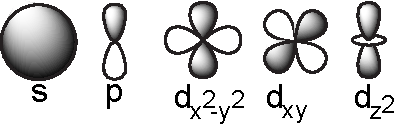
\includegraphics[width=105mm]{orbitals.pdf}
}

\frame{
	\frametitle{Atomové orbitaly}
	\begin{itemize}
	\item Orbital f - existuje sedm degenerovaných orbitalů typu f. Tyto orbitaly jsou obsazovány elektrony až u vnitřně přechodných prvků.
	\end{itemize}

	\begin{center}
	\adjincludegraphics[width=85mm]{forbitals.png}
	\url{https://commons.wikimedia.org/wiki/File:F\_orbital.png}
	Autor: \href{https://commons.wikimedia.org/wiki/User:A2569875}{A2569875}
	\end{center}
}

\frame{
	\frametitle{Molekulové orbitaly}
	\begin{itemize}
	\item Teorie LCAO-MO - Linear Combination of Atomic Orbitals - Molecular Orbital
	\item Molekulové orbitaly vznikají lieární kombinací atomových orbitalů
	\item Kombinací dvou AO vznikají dva MO - vazebný a protivazebný. Protivazebné orbitaly se označují hvězdičkou, např. $\sigma^*$
	\item Aby byl překryv úspěšný musí mít vlnové funkce orbitalů v místě překryvu stejná znaménka
	\item Protivazebný orbital má o jednu nodální plochu více než vazebný a pokud je obsazen elektronovým párem, snižuje řád vazby o jedna. Obsazený vazebný orbital naopak řád vazby zvyšuje.
	\item Vazba $\sigma$ - vzniká osovým překryvem orbitalů.
	\item Vazba $\pi$ - vzniká bočným překryvem orbitalů, je přítomna v násobných vazbách.
	\item Vazba $\delta$ - vzniká překryvem všech čtyř laloků d-orbitalu, je přítomna ve čtverné vazbě např. v \href{http://pubs.acs.org/doi/abs/10.1021/ic50025a015}{\ce{[Re2Cl8]^{2-}}}.
	\end{itemize}
}

\frame{
	\frametitle{Řád vazby}
	\begin{itemize}
	\item Řád vazby popisuje počet elektronových párů, které tvoří vazbu mezi atomy.
	\item Lze jej odvodit z Lewisovského vzorce molekuly nebo z diagramu MO.
	\end{itemize}

	\begin{center}
	\chemfig{H-[:52.24]\lewis{13,O}-[::-104.48]H}
	\raisebox{3.5ex}{\chemfig{\lewis{35,O}=C=\lewis{17,O}}}
	\end{center}

	\begin{itemize}
	\item Řád vazby lze spočítat z počtu elektronů ve vazebných a protivazebných orbitalech.
	\item $RV = \frac{vazebne\ elektrony - protivazebne\ elektrony}{2}$

	\item Neobsazené molekulové orbitaly neovlivňují ani řád vazby, ani energii systému.
	\end{itemize}

}

\frame{
	\frametitle{Literatura}
	\begin{enumerate}
	\item \href{http://www.chemguide.co.uk/atoms/properties/atomorbs.html}{www.chemguide.co.uk/atoms/properties/atomorbs.html}
	\item \href{http://chemed.chem.purdue.edu/genchem/topicreview/bp/ch8/mo.html}{Molecular Orbital Theory}
	\end{enumerate}
}

\end{document}